Diffuse

\begin{equation}
  l_{\rm rec} = E_{\rm Ly\alpha} f_{\rm rec} \dot{n}_{\rm rec} \left( \textbf{x}, z \right)
\end{equation}

\begin{equation}
  \dot{n}_{\rm rec} \left( \textbf{x}, z \right) = \alpha_{\rm A} n_{e} \left(z \right) n_{HII} \left(z \right)
\end{equation}

This is an equation $n_{e} = x_i \left( \textbf{x}, z \right) n_{b} \left( \textbf{x}, z \right) $

\begin{equation}
  n_{b} \left( \textbf{x}, z \right) = \bar{n}_{b, 0} \left( 1 + z\right)^3 \left[1 + \delta_{\rm nl} \left( \textbf{x}, z\right) \right]
\end{equation}

\begin{equation}
  \alpha_{\rm A} \approx 4.2 \times 10^{-13} \left( T_{\rm K} / 10^4 {\rm K} \right)^{-0.7} \left( 1 + z\right)^3 \left[\rm  cm^3 \ s^{-1} \right]
\end{equation}

\begin{equation}
I_{\rm rec, \nu} = y \left(z \right) d_A^2 \left(z \right) \frac{l_{\rm rec} \left( \textbf{x}, z \right)}{4 \pi d_L^2 \left( z \right)}
\end{equation}

Scattered

\begin{equation}
  I_{\nu} = \frac{6 E_{\text{Ly}\alpha}\, d_\textsc{a}^2 \left(z \right)}{\left( 1 + z\right)^2 d_\textsc{l}^2 \left( z \right)}\, J_{\alpha} \left( \textbf{x}, z \right)
\end{equation}

\begin{equation}
  \delta I_{\nu} \left(\textbf{x}, z \right) = \sum_i \frac{\nu I_{\nu, i} \left(\textbf{x}, z \right)}{\nu \bar{I}_{\nu} \left(z \right)} - 1
\end{equation}

\begin{figure}[ht]
	\centering
	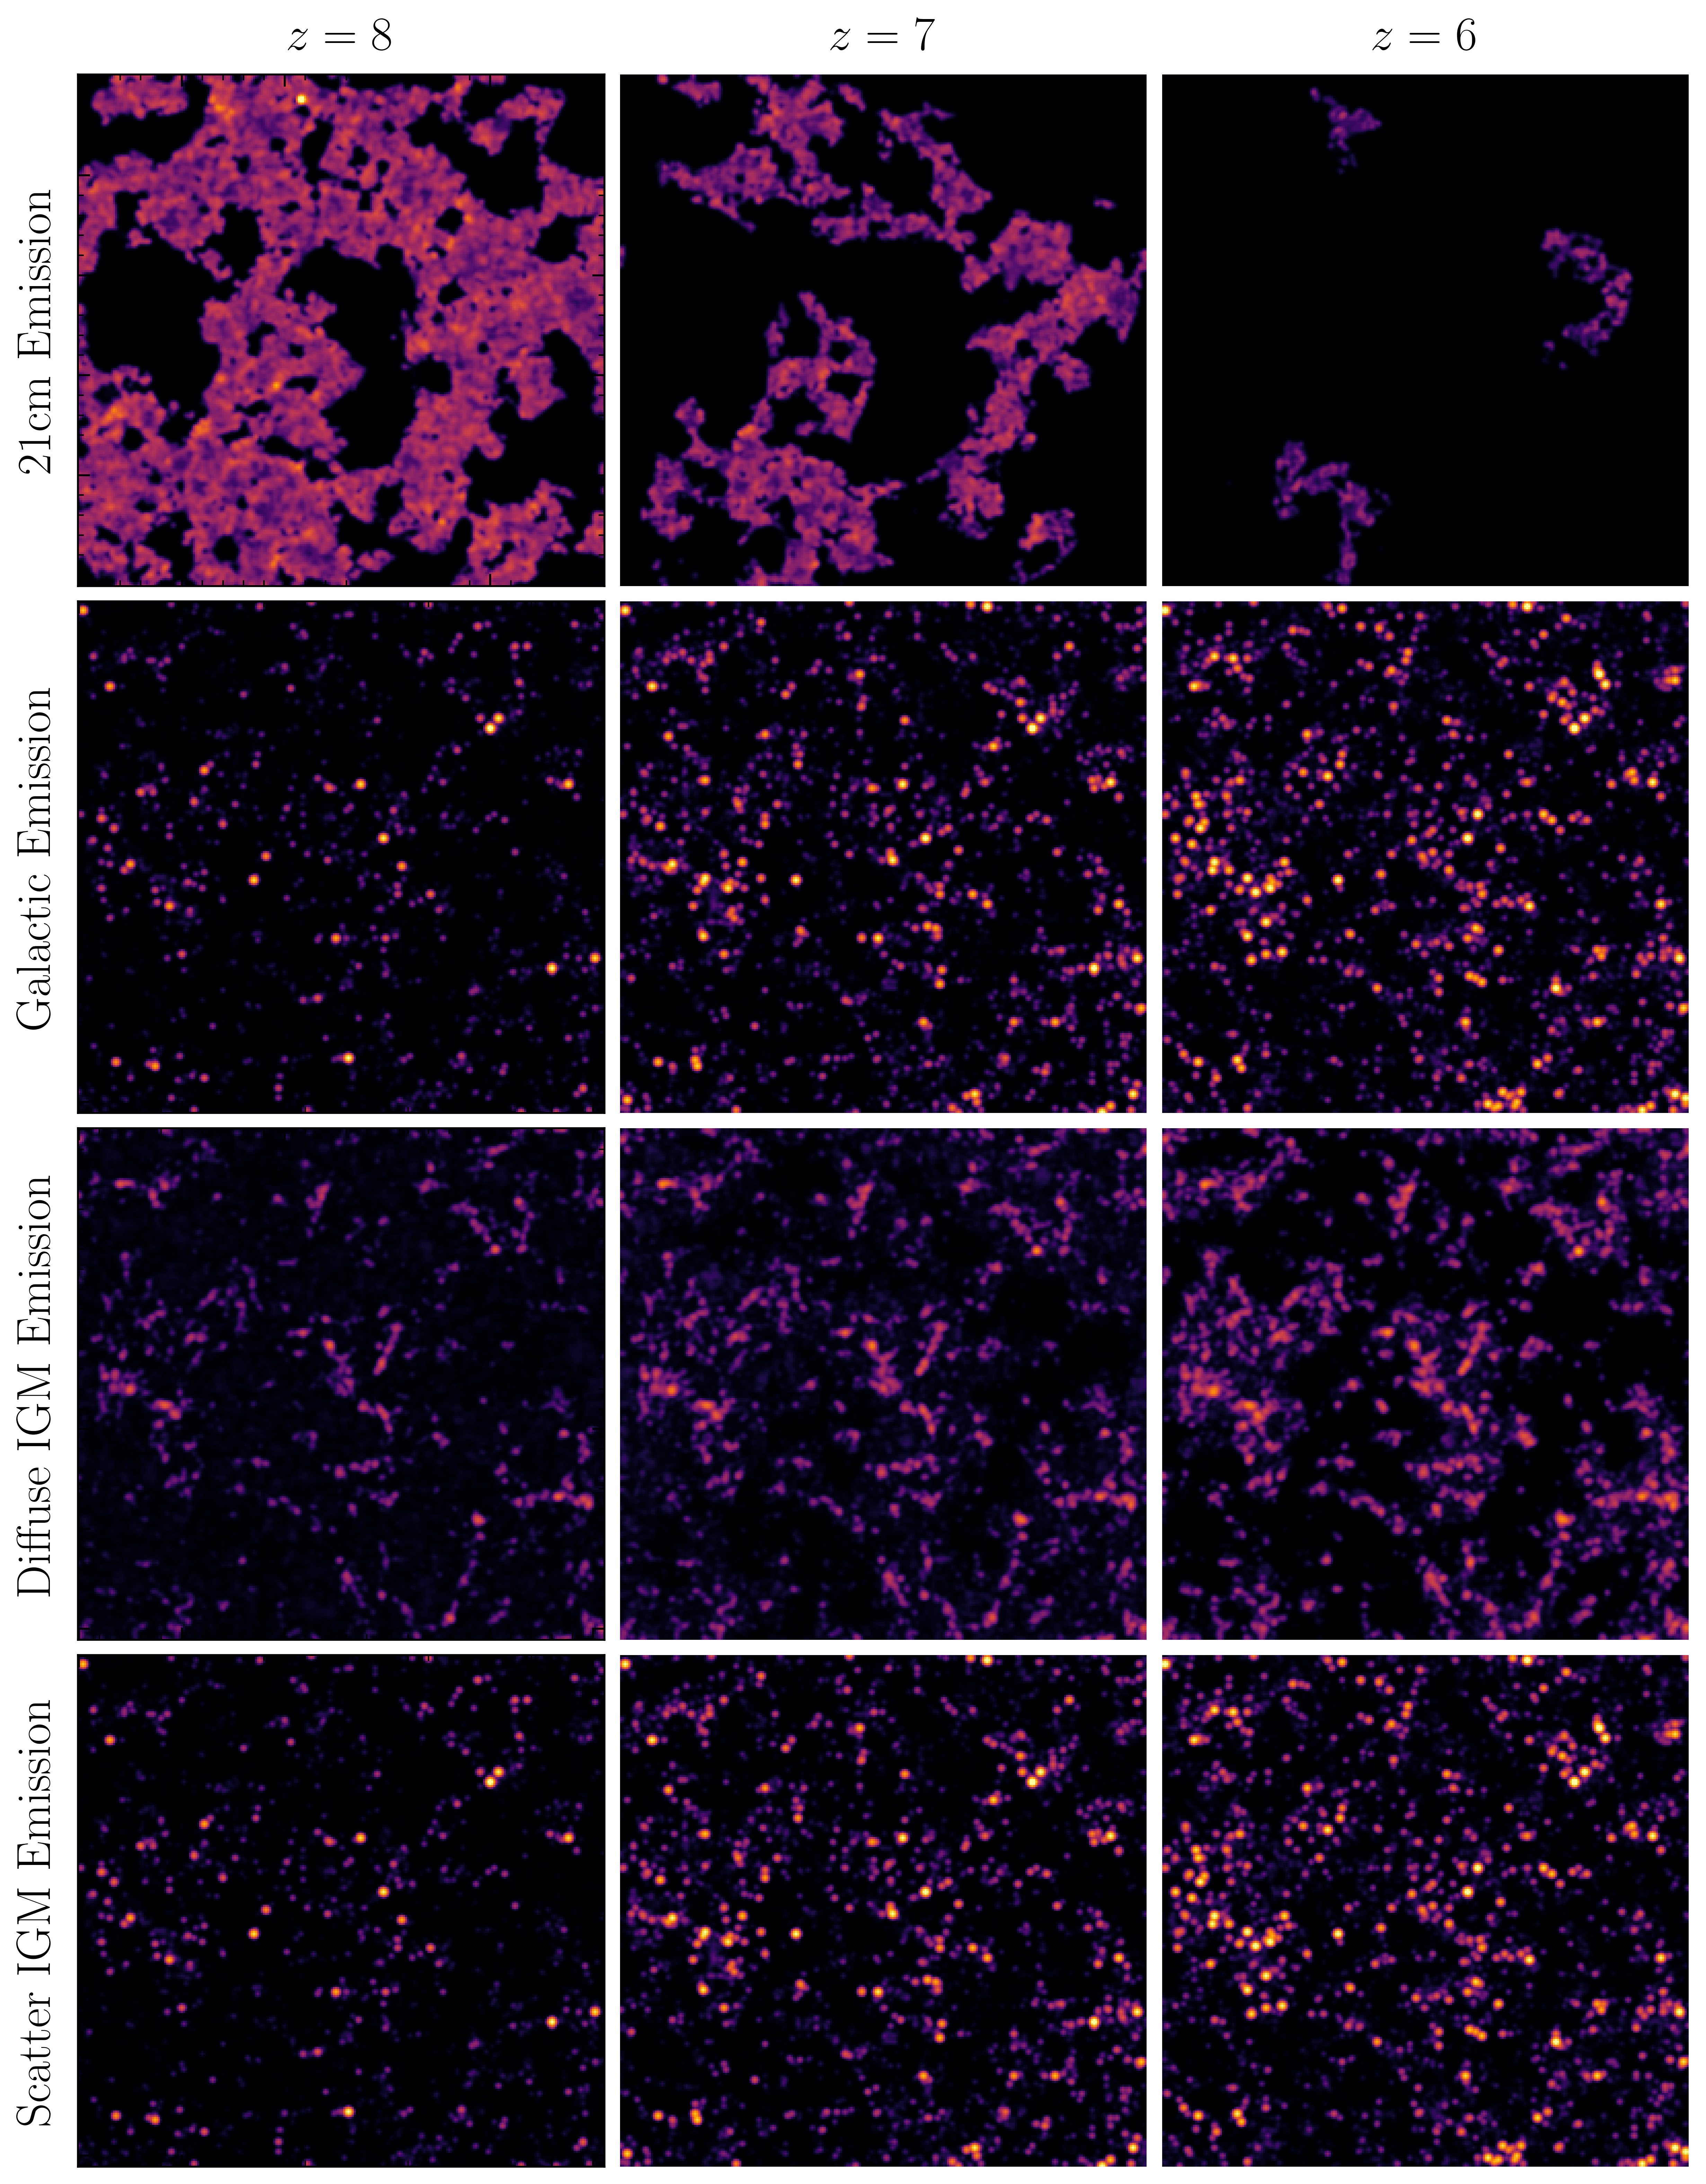
\includegraphics[width=1\textwidth]{sims.png}
	\caption[Simulated 21cm and Ly$\alpha$ emission]{Simulated 21cm and Ly$\alpha$ emission
	 as described in section blah. Each column represents simulated emission at different
	 redshift value.}
	\label{fig:sims}
\end{figure}
